\chapter{Project Scheduling and Planning}

\section{Project Timeline}

The project was executed over two semesters spanning approximately 10 months, divided into five phases (Table~\ref{tab:timeline}).

\begin{table}[H]
\centering
\caption{Project Timeline}
\vspace{6pt}
\begin{tabularx}{\textwidth}{|C{1cm}|X|L{2.8cm}|X|}
\hline
\textbf{Phase} & \textbf{Activities} & \textbf{Duration} & \textbf{Deliverables} \\
\hline
1 & Requirements gathering, literature review, SRS & Weeks 1--3 & SRS document \\
\hline
2 & System design, architecture, DB schema, wireframes & Weeks 4--6 & Design document \\
\hline
3 & Backend development: auth, interview, resume, payment APIs & Weeks 7--12 & Working REST API \\
\hline
4 & Frontend development, AI integration, coding module & Weeks 13--20 & Complete web app \\
\hline
5 & Testing, bug fixing, deployment, documentation & Weeks 21--24 & Deployed system \\
\hline
\end{tabularx}
\label{tab:timeline}
\end{table}

\section{Work Breakdown Structure}

\begin{enumerate}
  \item \textbf{WP1 -- Project Management:} Weekly meetings, Git version control, GitHub Issues tracking.
  \item \textbf{WP2 -- Backend Development:} Authentication, interview CRUD, resume pipeline, Gemini integration, Stripe, Socket.IO, admin APIs.
  \item \textbf{WP3 -- Frontend Development:} React components, routing, interview room, coding page, feedback page, dashboard.
  \item \textbf{WP4 -- AI Server Development:} FastAPI setup, MediaPipe video analysis, Librosa audio analysis, resume parsing.
  \item \textbf{WP5 -- Testing and Deployment:} Unit/integration testing, Vercel/Render deployment, MongoDB Atlas, CORS configuration.
\end{enumerate}

\section{Gantt Chart}

\begin{figure}[H]
\centering
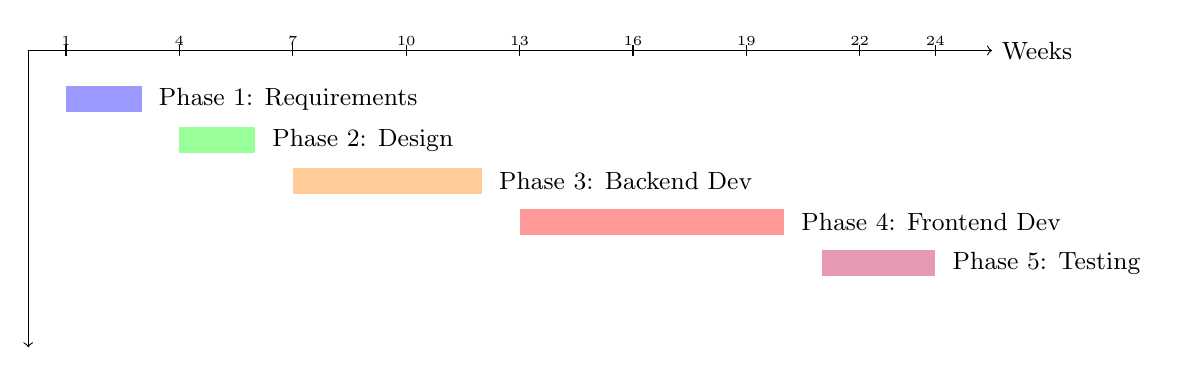
\begin{tikzpicture}[x=0.48cm, y=0.65cm]
  \draw[->] (0,0) -- (25.5,0) node[right, font=\small] {Weeks};
  \draw[->] (0,0) -- (0,-5.8);

  \foreach \w in {1,4,7,10,13,16,19,22,24} {
    \draw (\w,0.1) -- (\w,-0.1) node[above, font=\tiny] {\w};
  }

  \fill[blue!40]   (1,-0.7) rectangle (3,-1.2);
  \fill[green!40]  (4,-1.5) rectangle (6,-2.0);
  \fill[orange!40] (7,-2.3) rectangle (12,-2.8);
  \fill[red!40]    (13,-3.1) rectangle (20,-3.6);
  \fill[purple!40] (21,-3.9) rectangle (24,-4.4);

  \node[right, font=\small] at (3.2,-0.95)  {Phase 1: Requirements};
  \node[right, font=\small] at (6.2,-1.75)  {Phase 2: Design};
  \node[right, font=\small] at (12.2,-2.55) {Phase 3: Backend Dev};
  \node[right, font=\small] at (20.2,-3.35) {Phase 4: Frontend Dev};
  \node[right, font=\small] at (24.2,-4.15) {Phase 5: Testing};
\end{tikzpicture}
\caption{Project Gantt Chart}
\label{fig:gantt}
\end{figure}

\section{Resource Allocation}

\begin{table}[H]
\centering
\caption{Resource Allocation by Team Member}
\vspace{6pt}
\begin{tabularx}{\textwidth}{|L{3.5cm}|X|}
\hline
\textbf{Team Member} & \textbf{Primary Responsibilities} \\
\hline
\studentNamea & Backend API development, Gemini integration, deployment \\
\hline
\studentNameb & Frontend development, React components, state management \\
\hline
\studentNamec & AI server development, MediaPipe, audio analysis \\
\hline
\studentNamed & Database design, testing, documentation \\
\hline
\end{tabularx}
\label{tab:resources}
\end{table}

\section{Risk Management}

\begin{table}[H]
\centering
\caption{Risk Register}
\vspace{6pt}
\begin{tabularx}{\textwidth}{|X|C{1.8cm}|C{1.5cm}|X|}
\hline
\textbf{Risk} & \textbf{Probability} & \textbf{Impact} & \textbf{Mitigation} \\
\hline
Gemini API rate limits & Medium & High & Implement fallback questions; cache responses \\
\hline
Render free tier OOM & High & High & Build TypeScript in build phase; strip heavy Python deps \\
\hline
Piston API downtime & Medium & Medium & Implement local fallback executor \\
\hline
MongoDB Atlas IP blocking & Low & High & Use 0.0.0.0/0 whitelist; set Google DNS \\
\hline
Browser camera permission denied & Medium & Medium & Graceful audio-only fallback \\
\hline
\end{tabularx}
\label{tab:risks}
\end{table}
